\section{离散问题}
\label{sec:pdenum-discrete}

一个定义在区间上的函数有无穷多个值，怎样只用有限个数把它留下来？答案不止一种，不同的答案决定了后面的方程长什么样。全章的第一个例子是
\begin{equation}
 -u''=\pi^2\sin(\pi x)\quad\text{于}\ (0,1),\qquad u(0)=0,\quad u(1)=1,
 \label{eq:pdenum-model}
\end{equation}
它的解是
\begin{equation}
 u(x)=\sin(\pi x)+x .
 \label{eq:pdenum-model-exact}
\end{equation}

\paragraph{三类未知量}
把$[0,1]$等分成四段，步长$h=1/4$，节点$x_j=jh$。下面三种记录方式都只用几个数，含义却不同，图~\ref{fig:pdenum-three-unknowns}把它们画在同一个解上。

第一种记录节点上的值$U_j\approx u(x_j)$。这串数称为\term{网格函数}（grid function），它只在节点上有定义，节点之间是什么并不规定。有限差分方法的未知量就是它。

第二种记录一组基函数的系数$c_j$，把近似写成$u_h(x)=\sum_jc_j\varphi_j(x)$。$u_h$是定义在整个区间上的函数，可以求导、积分。若每个$\varphi_j$在节点$x_j$处为$1$、在其他节点处为$0$，系数恰好等于节点值，但它们的身份仍然是函数的坐标。有限元方法的未知量是它。

第三种把区间分成单元$C_j$，记录每个单元上的平均
\begin{equation}
 \bar{u}_j=\frac{1}{\lvert C_j\rvert}\int_{C_j}u\,\mathrm{d}x .
 \label{eq:pdenum-cell-average}
\end{equation}
它不是任何一点的值，而是这个单元里的总量除以长度。有限体积方法的未知量是它。

\begin{BookInlineFigure}
 \centering
 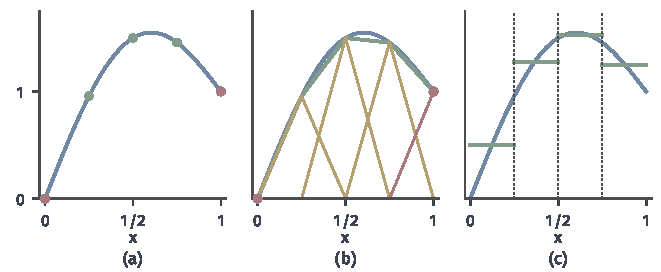
\includegraphics[width=112mm]{figures/06-differential-equations/02-partial-differential-equations/matplotlib/pdenum-three-unknowns/figure.pdf}
 \caption{同一个解$u=\sin(\pi x)+x$（蓝）的三种记录方式，$h=1/4$，红点是边值。(a)内部节点上的值（绿点）。(b)帽函数按节点值加权（黄线，右端红线是边界帽函数），其和是绿色折线。(c)四个单元上的平均（绿色水平线），虚线是单元界面。}
 \label{fig:pdenum-three-unknowns}
\end{BookInlineFigure}

把函数看成无限维向量，这三种做法都是在挑选有限个坐标：节点值是“按位置取样”，基函数系数是“在子空间里找坐标”，单元平均是“按小块累计”。类比到此为止，因为这三种坐标并不是同一个向量的不同分量，它们彼此之间相差一个与$h$有关的量。

例如在第一个单元$[0,1/4]$上，解的平均值由积分算出：
\[
 \bar{u}_1=4\int_0^{1/4}\bigl(\sin(\pi x)+x\bigr)\,\mathrm{d}x=\frac{4}{\pi}\Bigl(1-\frac{\sqrt2}{2}\Bigr)+\frac18\approx0.4979,
\]
而单元中点的值是$u(1/8)\approx0.5077$。比较数值解时必须说清比较的是哪一种量。

\paragraph{边界和初值怎样进入}
未知量选定后，还要说明已知数据放在哪里。Dirichlet边值是已知的节点值，它不再是未知量，而是把含它的项移到方程右端，右端因此带上边界数据。第~\ref{sec:pdenum-elliptic-fd}小节和第~\ref{sec:pdenum-weak-galerkin}小节会分别算出这一项。

Neumann条件和Robin条件规定的是边界通量。在弱形式和有限体积方法中，通量本来就在方程里出现，这些条件直接写进边界那一项；在差分格式中，则要用边界附近的差商或虚拟节点表达它们。

演化方程的初值$u_0$给出第一层数据，要按未知量的身份换算：差分取节点值，有限元取插值或投影，有限体积取单元平均。初值若不连续，这几种换算的差别并不小，后面的激波例子会用到单元平均。

\paragraph{三步离散，三份误差}
对演化方程，从$u$到屏幕上的数字要经过三步（图~\ref{fig:pdenum-error-pipeline}）。空间离散把场换成有限个未知量，得到第~\ref{chap:ode-numerical-methods}章讨论的常微分方程组；时间推进把它变成逐层的代数关系；每一层若含隐式方程，还要由有限精度的线性代数算出来。

\begin{BookInlineFigure}
 \centering
 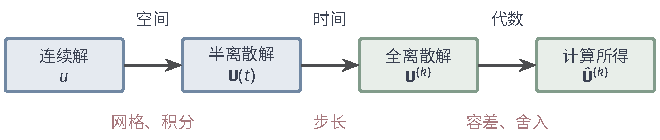
\includegraphics[width=112mm]{figures/06-differential-equations/02-partial-differential-equations/tikz/pdenum-error-pipeline/figure.pdf}
 \caption{从连续解到计算结果的三步。每个箭头引入一份误差，下方红字是控制它的主要因素。椭圆问题没有时间步，只有空间和代数两步。}
 \label{fig:pdenum-error-pipeline}
\end{BookInlineFigure}

记半离散解为$\bm{U}(t)$，全离散解为$\bm{U}^{(k)}$，实际算出的为$\widehat{\bm{U}}^{(k)}$，$\bm{R}_hu$表示把连续解按未知量的身份换算成离散向量。总误差分成三段：
\begin{equation}
 \begin{aligned}
 \bm{R}_hu(t_k)-\widehat{\bm{U}}^{(k)}
 &=\bigl(\bm{R}_hu(t_k)-\bm{U}(t_k)\bigr)\\
 &\quad+\bigl(\bm{U}(t_k)-\bm{U}^{(k)}\bigr)
 +\bigl(\bm{U}^{(k)}-\widehat{\bm{U}}^{(k)}\bigr).
 \end{aligned}
 \label{eq:pdenum-error-split}
\end{equation}

这样拆的好处是每一段可以单独控制，也可以单独检验。加密网格却不减小时间步，误差会停在时间误差的水平上；线性方程解得不够精确，误差会停在代数误差的水平上。第~\ref{sec:pdenum-error-cost}节会实际看到这两种停滞。

和常微分方程不同，这里步长变小时，向量$\bm{U}$的维数也在变。不同$h$对应的误差要能比较，范数必须随网格换算，比如$\lVert\bm{v}\rVert_{2,h}=(h\sum_jv_j^2)^{1/2}$相当于$L^2$范数，而$\lVert\bm{v}\rVert_\infty$相当于最大模。不带因子$h$的欧氏范数会随未知量增多而变大，不能用来比较。
